\documentclass[12pt]{article}

\usepackage[margin=1in]{geometry}
\usepackage{setspace}
\usepackage{graphicx}
\usepackage{booktabs}
\usepackage{amsmath}
\usepackage{float}
\usepackage{hyperref}
\hypersetup{hidelinks}

\onehalfspacing
\setlength{\parskip}{0.15em}
\setlength{\parindent}{0em}

\title{Dimension Reduction of an ERCOT Battery Fleet\\
\large PCA, Proper Orthogonal Decomposition, and a Low-Rank SVD}
\author{Jonathan Kazmaier}
\date{October 27, 2026}

\begin{document}
\maketitle
\vspace{-1.2em}

\section{The setting}

ERCOT operates the electric grid for most of Texas and runs its wholesale electricity market.
About every five minutes it chooses which power plants and batteries produce or absorb power, so that supply matches demand.
The wires do not store electricity.
A megawatt is a rate of power.
One megawatt for an hour serves roughly a thousand homes at ordinary use, and a few thousand megawatts is a few percent of Texas on a hot afternoon.

In July the largest use is air conditioning.
Demand rises through the afternoon and stays high into the evening, when people are home and buildings are still hot.
That stretch is the evening peak.
Solar farms produce the most late in the morning and around noon, then fall off as the sun drops.
The tight hours are the overlap: air conditioners are still running, and the solar supply is leaving.

A grid battery stores electrical energy.
Charging draws power off the grid.
Discharging sends stored energy back for customers to use.
In a Texas July, power is abundant and cheap in the late morning, when solar output is high, and scarce and expensive at the evening peak.
A battery charges in the first window and discharges in the second.
Over a full day the two largely cancel, so a busy battery can still average near zero.
Negative megawatts in this report mean charging.
Positive megawatts mean discharging.
The fleet is every battery added together.
The batteries see the same sun and the same evening demand, which is why a few shared patterns can describe the sum.
They still differ in size.
Some are offline, and some are held in reserve instead of cycling every day, which is why one battery is harder to rebuild than the total.

\section{The data}

Each row of the matrix is one hour and each column is one battery.
The entry is that hour's average metered output, in megawatts.
The source is \texttt{fact\_esr\_soc}, where ERCOT publishes each battery's meter about 60 days later.
The window is 1--28 July 2026.
A reading is kept when the status is \texttt{ON} or \texttt{ONTEST}: the battery was online in normal service or on a test run.
A battery stays in the matrix if it was online for at least 24 hours and its typical power rating is at least 5~MW.
That rating, the high sustained limit, is the most power it may push onto the grid or pull off it.
An hour with no online reading is 0~MW.
The matrix is 672 hours by 297 batteries.

Each hour is one snapshot of the same batteries.
Proper orthogonal decomposition finds the snapshot patterns with the most energy.
Principal component analysis is the same calculation with hours as observations and batteries as variables.
The median battery is rated 50~MW.
Together, the fleet averaged 255~MW of charging, with an hour-to-hour standard deviation of $3{,}357$~MW.
On the average day the 9:00 hour is about $7{,}169$~MW of charging and the 20:00 hour is about $7{,}843$~MW of discharging.
The sign change falls in the 18:00 hour.

\section{The code}

The code and this report are posted here:

\url{https://github.com/JonKazz/battery-fleet-pca}

\texttt{01\_fleet\_pca.py} implements both procedures.
\texttt{pca\_reconstruct} in that file is section 10.6.
\texttt{truncated\_svd} in that file is section 10.4.
\texttt{02\_figures.py} draws the two figures from the tables in \texttt{results/}.

The PCA routine has five steps.
Subtract each battery's mean over the 672 hours.
Optionally divide by its sample standard deviation, with $n-1$ in the denominator.
A standard deviation below $10^{-8}$ is replaced by 1.
Form the $297 \times 297$ covariance $(1/(n-1)) A^{\mathsf T} A$.
Keep the $k$ leading eigenvectors, project, then undo the scaling and add the means back.
Every score below is in megawatts, after that last step.

The SVD routine does not center or scale.
It keeps the $k$ largest singular values of the raw megawatt matrix and the matching singular vectors.
That product is the best rank-$k$ approximation in the Frobenius norm.

Three scores are used.
Relative Frobenius error is the size of the residual divided by the size of the original matrix.
Fleet RMSE and fleet $R^{2}$ compare the hour-by-hour sum of all batteries with the same sum from the reconstruction.
Mean unit RMSE averages the time-series error of each battery, so a small battery counts once.

\section{What the steps change}

The matrix was decomposed raw, after mean subtraction, and after mean subtraction plus standardization.
Table~\ref{tab:errors} samples the ranks.
Figure~\ref{fig:error} shows every rank from 1 to 40.

\begin{table}[H]
\centering
\singlespacing
\caption{Share of energy in the decomposed matrix, and relative error after the result is returned to megawatts.}
\label{tab:errors}
\small
\resizebox{\textwidth}{!}{%
\begin{tabular}{rrrrr}
\toprule
$k$ & Energy, raw SVD & Rel.\ error, raw SVD & Rel.\ error, centered PCA & Rel.\ error, standardized PCA \\
\midrule
1  & 0.538 & 0.680 & 0.680 & 0.692 \\
5  & 0.647 & 0.594 & 0.594 & 0.641 \\
12 & 0.753 & 0.497 & 0.497 & 0.583 \\
40 & 0.914 & 0.293 & 0.293 & 0.472 \\
\bottomrule
\end{tabular}}
\end{table}

Mean subtraction does not matter here.
The median battery's monthly mean is 0.5~MW, because charge and discharge cancel.
At every rank the centered PCA and the raw SVD agree to three digits.
At $k = 1$ the fleet RMSE is 249~MW without centering and 248~MW with it.
The mean was already almost zero, so removing it does not free a component.

Standardization does matter, and it makes the megawatt rebuild worse.
Dividing by the standard deviation gives a 10~MW battery the same vote as a 100~MW battery.
The first component then holds 41\% of the scaled energy, against 54\% of the raw megawatt energy.
Back in megawatts, the $k = 1$ fleet RMSE rises from 249~MW to 451~MW, and the fleet $R^{2}$ falls from 0.994 to 0.982.
At $k = 40$ the relative error is 0.47 with standardization and 0.29 without it.
Standardization answers ``what does a typical battery do.''
The fleet total is weighted by size, so the large batteries are the fleet.

Section 10.4 and section 10.6 are the same decomposition applied to different matrices.
The truncated SVD is optimal for the matrix it receives.
On these data the column means are negligible, so the best rank-$k$ approximation of the raw matrix already matches centered PCA.
The curves sit on top of each other in both figures.
They separate once each column is scaled to variance one.
That standardized problem is optimal for correlations.
Putting the megawatts back at the end does not make it optimal for megawatts.
A check on the code: a truncated SVD of the centered matrix reproduces the centered-PCA column of Table~\ref{tab:errors}.
For centered data, the leading covariance eigenvectors are the right singular vectors.

\section{How low can the rank be?}

For the fleet total, one component is enough.
The raw SVD and the centered PCA at $k = 1$ have fleet $R^{2} = 0.994$.
Figure~\ref{fig:day} averages that reconstruction over the 28 days.
The 9:00 charge returns as $7{,}169$~MW, matching the actual average, and the 20:00 discharge returns as $7{,}647$~MW against $7{,}843$~MW.
That curve is the dominant mode: deep charging late in the morning, a shallow charge through the afternoon, and discharge through the evening.
The combined fleet schedule needs a single component.

\begin{figure}[H]
\centering
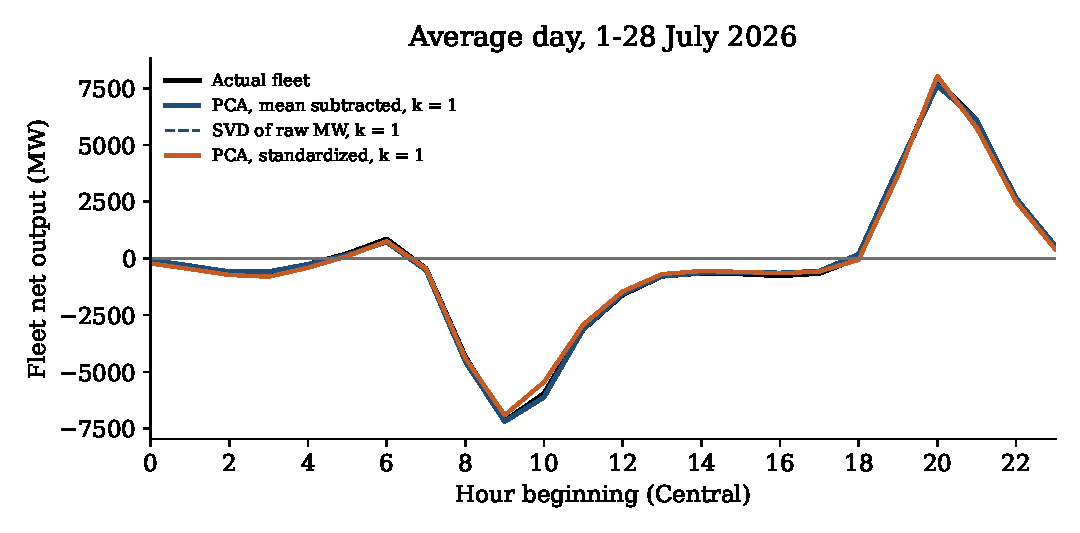
\includegraphics[width=0.88\textwidth]{results/diurnal_k1.pdf}
\caption{Average fleet output by hour. Negative means charging. Centered PCA and the raw SVD overlap. Standardized PCA is shallow on the morning charge and high on the evening peak.}
\label{fig:day}
\end{figure}

One component does not recover each battery.
It holds 54\% of the megawatt energy, and the relative error on the whole matrix is still 0.68.
The median battery's correlation with the fleet total is 0.65, and only 38\% of batteries exceed 0.7.
At $k = 1$ the average battery is off by 11~MW, against a median rating of 50~MW.
Twelve components bring the relative error to 0.50.
Forty bring it to 0.29 and the mean unit error to 5.5~MW.
Forty out of 297 is still a large reduction, and it is where a per-battery reconstruction becomes useful.
Figure~\ref{fig:error} falls quickly through the first component and then flattens: later components are real, and each buys less than the shared daily mode.

\begin{figure}[H]
\centering
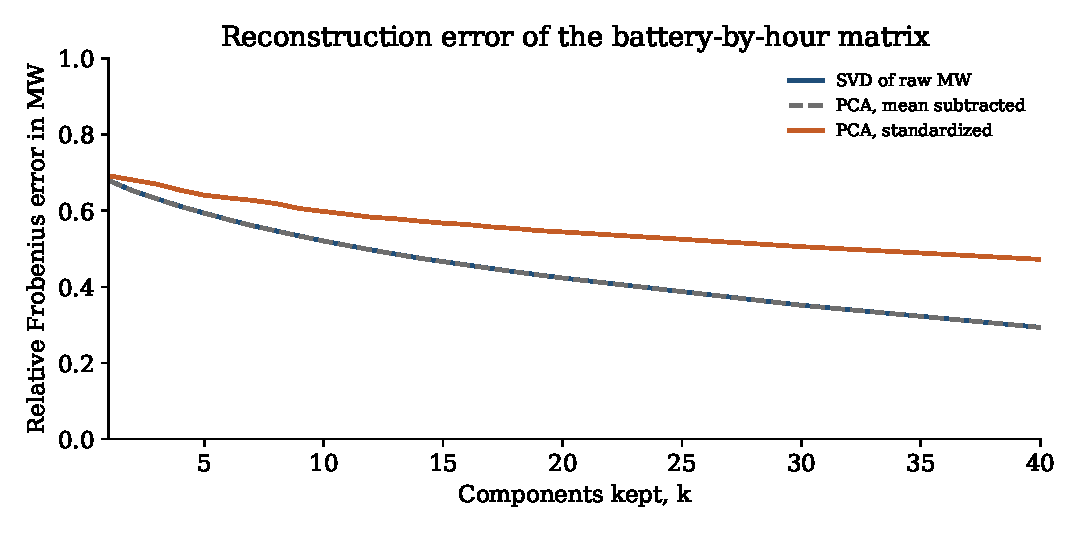
\includegraphics[width=0.88\textwidth]{results/error_vs_k.pdf}
\caption{Relative error of the $672 \times 297$ matrix, in megawatts. The raw SVD and centered PCA overlap. Standardization stays higher at every rank.}
\label{fig:error}
\end{figure}

The fleet schedule is rank one.
Mean subtraction changes nothing, and standardization hands the fit to smaller units.
Rebuilding each battery takes a few dozen components.

\end{document}
